\section*{הקדמה}

נתחיל עם קצת רקע: החוברת הזאת היא חוברת עם מנגינות לנגינה על כלי פריטה קטנטן שנקרא „אוּקוּלֶלֶה” (השם הזה מגיע משפה שנקראת הוואיאית, והמשמעות של  השם \L{{\fontspec{Gentium}ʻ}ukulele} בה היא „פרעוש קופץ”). החוברת מיועדת למתחילים, מה שמתבטא בכמה אופנים:
\begin{itemize}
	\item הבחירה במנגינות מוכרות, חלקן שירים ידועים בעברית. לא כולן בהכרח „הלחם והטחינה” של כולם, אבל אני די בטוח שלפחות חלק תזהו.
	\item החוברת כוללת את הקו המלודי של המנגינות, ולא ליווי באקורדים, שהם לא שקופים להבנה.
	\item עיבדתי את המנגינות כך שבכל רגע נתון פורטים רק על מיתר אחד (מונופוניה). אחרי שתתאמנו על כל המנגינות שבחוברת תהיו מוכנים לגמרי לנגן כמה קולות (פוליפוניה).
	\item אופן ההצגה: בנוסף לסימון תווים בשיטה המערבית הרגילה לפי גובה הצליל, מצורפת טבלטורה. הטבלטורה מסמנת בדיוק על איזה סריג ללחוץ ועל איזה מיתר לפרוט\footnote{ולכן היא מתאימה לאוקוללה לפי הכיוון הרגיל בלבד, ולא לכלים אחרים.}. באופן כזה, כשהתווים הרגילים והטבלטורה נמצאים אחד מעל השני, מי שיודעים לקרוא תווים יכולים לקרוא אותם, וכולם יכולים לנגן לפי הטבלטורה.
\end{itemize}



\subsection*{כיוון}

אמרנו שלאוקוללה ארבעה מיתרים. הם מכוונים באופן קצת מוזר: לא לפי גובה הצליל כמו ברוב כלי המיתר, אלא בסדר אחר. המיתר הראשון\footnote{הקרוב ביותר אליכם כשאתר מחזיקים את הצוואר בצד שמאל.} מכוון בכיוון הרגיל לסול (\L{G}), הבא בתור לדו (\L{C}) באותה האוקטבה, ולאחריהם מי (\L{E}) ולה (\L{A}). ככה:

\begin{center}
	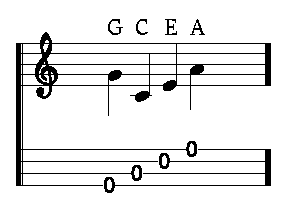
\includegraphics[height=3cm]{agordo.eps}
\end{center}

הדרך הכי קלה לכוון את האוקוללה בעזרת מכשיר כיוון אלקטרוני שמצמידים בתופסן לקצה האוקוללה. חשוב שתשיגו מכוון שלא מותאם לגיטרה בלבד אלא כזה שהוא כללי.



\subsection*{איך קוראים טבלטורה?}

נכון שלאוקוללה יש ארבעה מיתרים? אז לטבלטורה יש ארבע שורות, שמייצגות את ארבעת המיתרים כשמסתכלים מלמעלה והצוואר נמצא בצד שמאל שלכם. ימניים פורטים עם יד ימין ולוחצים בין הסריגים ביד שמאל; שמאליים מנגנים ככה או הפוך: מחזיקים את האוקוללה כשהצוואר בצד ימין, ופורטים עם יד שמאל ולוחצים בין הסריגים ביד ימין (ואז גם קוראים את הטבלטורה הפוך…).

קוראים משמאל לימין, וכשיש מספר אז לוחצים בין הסריגים במיתר המתאים ופורטים עליו. 0 מסמן פריטה על מיתר פתוח, בלי ללחוץ ביד השניה; 1 מסמן ללחוץ על המיתר לפני הסריג הראשון ולפרוט עליו; 2 לפני הסריג השני, וכן הלאה. סידרתי את הטבלטורה כך שתמיד יופיעו מספרים נמוכים ככל האפשר.

הסימון של משך הצליל מצויין רק בתווים, באופן רגיל: \symbolglyph{𝅝} מסמן משך שלם (\L{1}), \symbolglyph{𝅗𝅥} מסמן חצי (\L{½}), \symbolglyph{𝅘𝅥} מסמן רבע (\L{¼}), ו־\symbolglyph{𝅘𝅥𝅮} או \symbolglyph{♫} מסמנים שמינית (\L{⅛}); המקבילות של ההפסקות הן \symbolglyph{𝄻}, \symbolglyph{𝄼}, \symbolglyph{𝄽} ו־\symbolglyph{𝄾}, בהתאמה.

חזרות מסומנות ב־\symbolglyph{𝄆} ו־\symbolglyph{𝄇}. כשיש הבדל בין החזרה הראשונה והשניה משמש סימון \symbolglyph{⌜} ממוספר מעל התיבות השונות.

רוצים לוודא שהבנתם? הנה ההתחלה של „יונתן הקטן”. תנסו לראות אם זה מה שיוצא לכם כשאתם מנגנים:

\begin{center}
	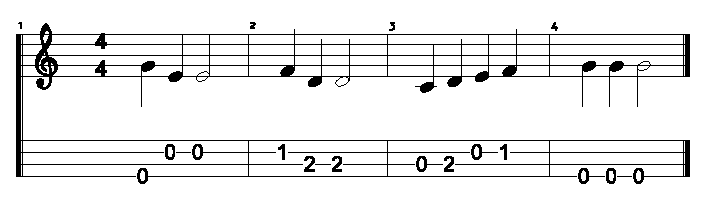
\includegraphics[height=3cm]{jon.eps}
\end{center}


\subsection*{מידע נוסף ויצירת קשר}

האתר של החוברת הוא \url{http://xpr.digitalwords.net/ukulele}; בקוד \L{QR}:

\begin{center}
	
\includegraphics[width=2cm]{retejo.png}
\end{center}

באתר נמצאים כל קבצי המקור של החוברת, כמו גם קובץ מוכן להדפסה (אם תרצו ליצור עותק נוסף או לקרוא במחשב). 

*** http://www.tuxguitar.com.ar/

***
***מידי+מקור (שאפשר לשמוע עם סימון גרפי)
